% 10min
\pentry{平面直角坐标系,矢量}
\begin{figure}[h]
\centering
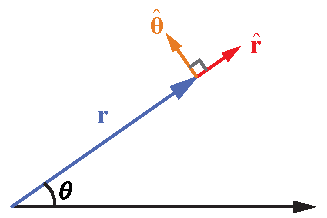
\includegraphics[width=6cm]{./figures/Polar.pdf}
\caption{极坐标系和两个单位矢量}
\end{figure}
在平面上上取一个点作为极点,过极点的一条轴作为极轴.选定极轴的正方向,规定单位长度.该平面上某点与原点连成的线段叫做\textbf{极径},其长度一般用 $r$ (或 $p$ )表示.若 $r$ 为负值,则表示反方向的长度.极径与极轴的夹角叫做极角(规定逆时针旋转极角增加,顺时针旋转则减少),用 $\theta $ 表示.若 $\theta $ 为负值,则表示从极轴开始延顺时针方向转动 $\abs{\theta}$ 角. $\theta $ 的值通常表示成弧度.于是任何一点都可以用两个有序实数 $(r,\theta)$ 来表示其在该平面上的位置,这就是一个点的\textbf{极坐标}.

一般以坐标名上面加单位矢量符号表示该坐标对应的单位矢量.例如直角坐标系中, $\uvec x$ (有时也记为 $\uvec i$ )是 $x$ 坐标增加方向的单位矢量.所以在极坐标中,定义 $\uvec r$ 为 $r$ 增加的方向的单位矢量, $\uvec \theta $ 为 $\theta $ 坐标增加方向的单位矢量(即 $\uvec r$ 逆时针旋转 $\pi/2$ 的方向).必须注意的是, $\uvec r$ 与 $\uvec \theta $ 互相垂直,构成一对\textbf{单位正交基底},平面上的任意向量都可以正交分解到这两个方向上.通常把 $\uvec r$ 的方向叫做\textbf{径向},把 $\uvec \theta $ 的方向叫做\textbf{法向}.

\begin{mdframed} \textbf{拓展阅读\ }极坐标中单位矢量的偏导%未完成:引用
,正交曲线坐标系%未完成:引用
\end{mdframed}





































